\documentclass[12pt,letterpaper]{article}
\usepackage{graphicx}
\usepackage{ifpdf}

\usepackage{multicol}
\usepackage{tikz}

\usepackage{amssymb}
\usepackage{amsmath}

\usepackage{hyperref}

\usepackage[spanish]{babel}

\usepackage{fancyhdr}
 
\pagestyle{fancy}
\fancyhf{}
\rhead{Isaac Ayala Lozano\\194520009\\\#2}
\lhead{}

\title{Notes on System Modeling}
\author{Isaac Ayala Lozano}
\date{}
    
\begin{document}
% \maketitle
\pagenumbering{gobble}

\begin{figure}
 \centering
 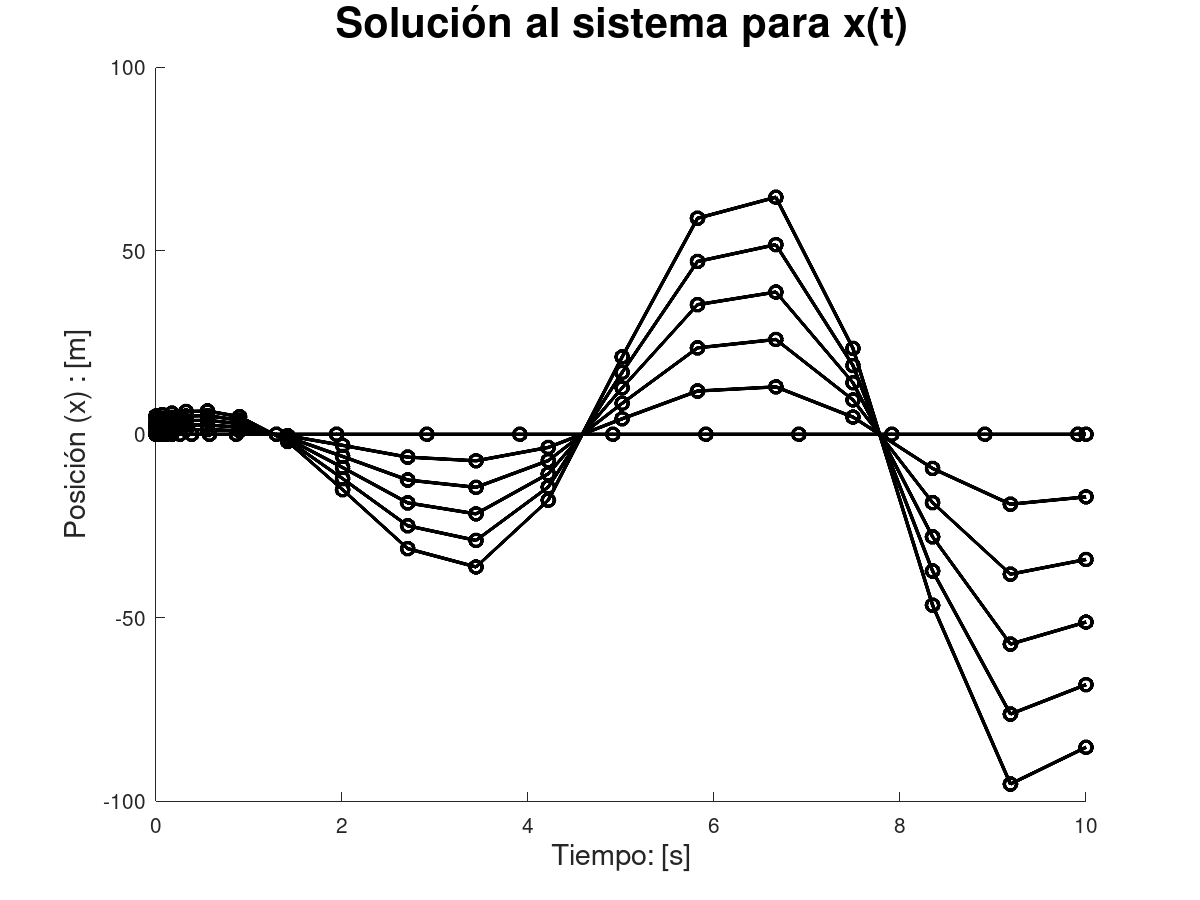
\includegraphics[scale=0.2]{img/fig01.png}
 % fig01.png: 1200x900 px, 72dpi, 42.33x31.75 cm, bb=0 0 1200 900
 \caption{Gráfica de $x(t)$.}
\end{figure}

\begin{figure}
 \centering
 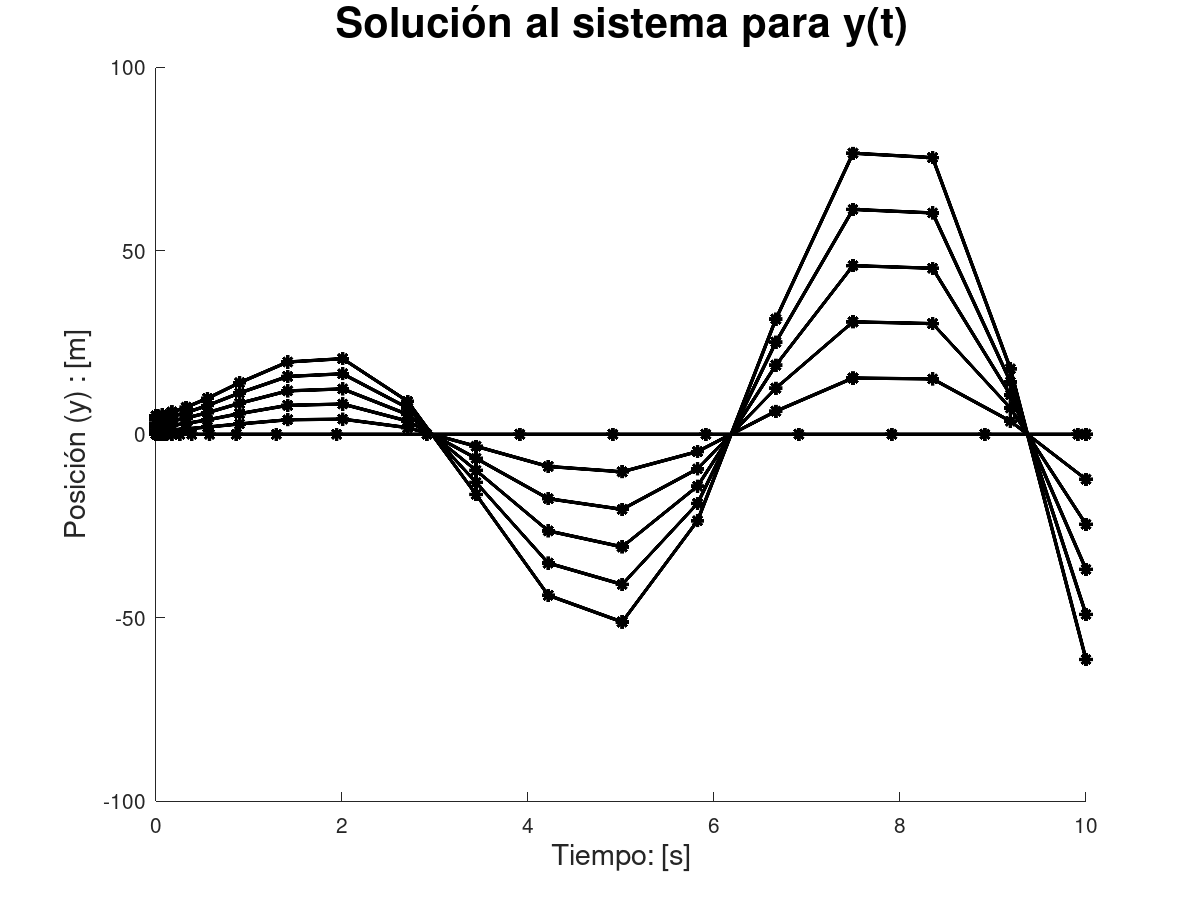
\includegraphics[scale=0.2]{img/fig02.png}
 % fig01.png: 1200x900 px, 72dpi, 42.33x31.75 cm, bb=0 0 1200 900
 \caption{Gráfica de $y(t)$.}
\end{figure}

\begin{figure}
 \centering
 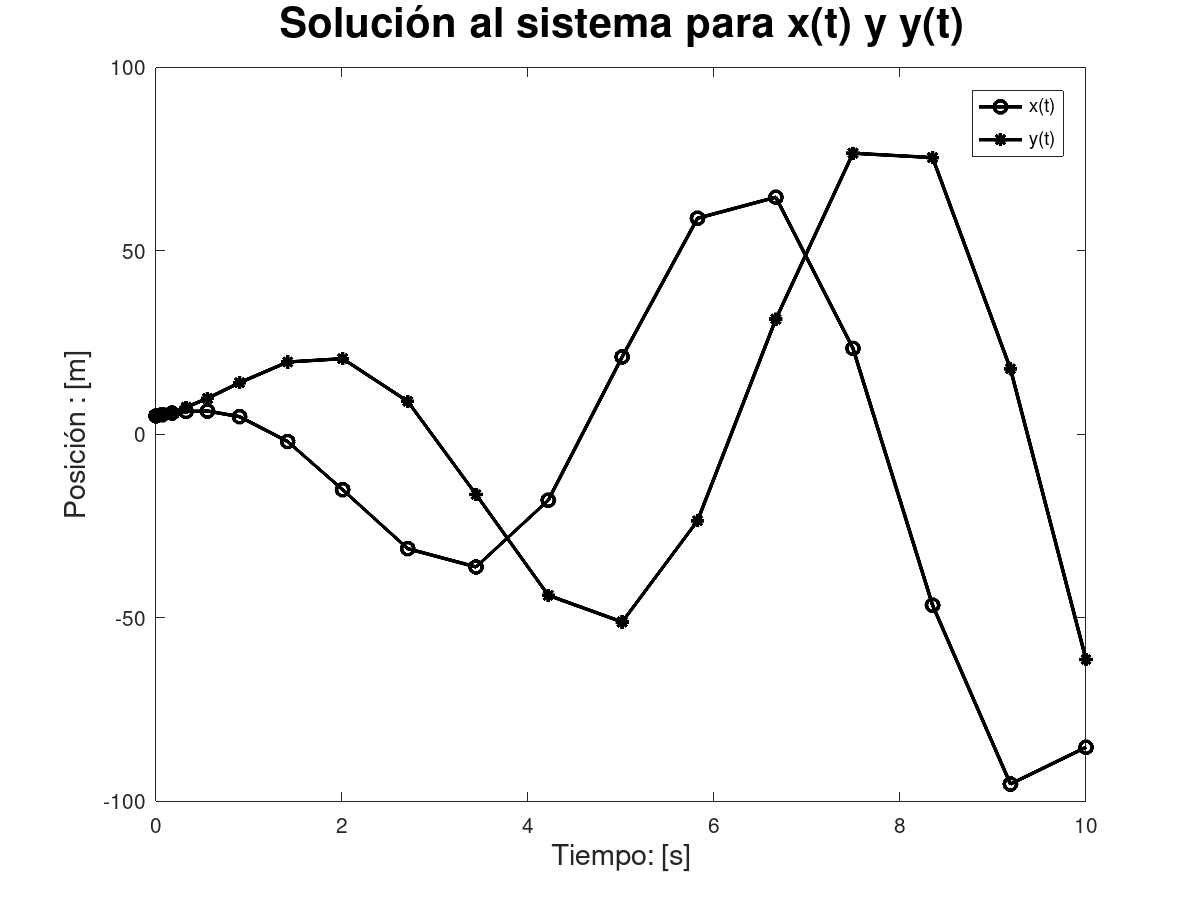
\includegraphics[scale=0.2]{img/fig03.png}
 % fig01.png: 1200x900 px, 72dpi, 42.33x31.75 cm, bb=0 0 1200 900
 \caption{Comparación de $x(t)$ y $y(t)$ con respecto al tiempo.}
\end{figure}

\begin{figure}
 \centering
 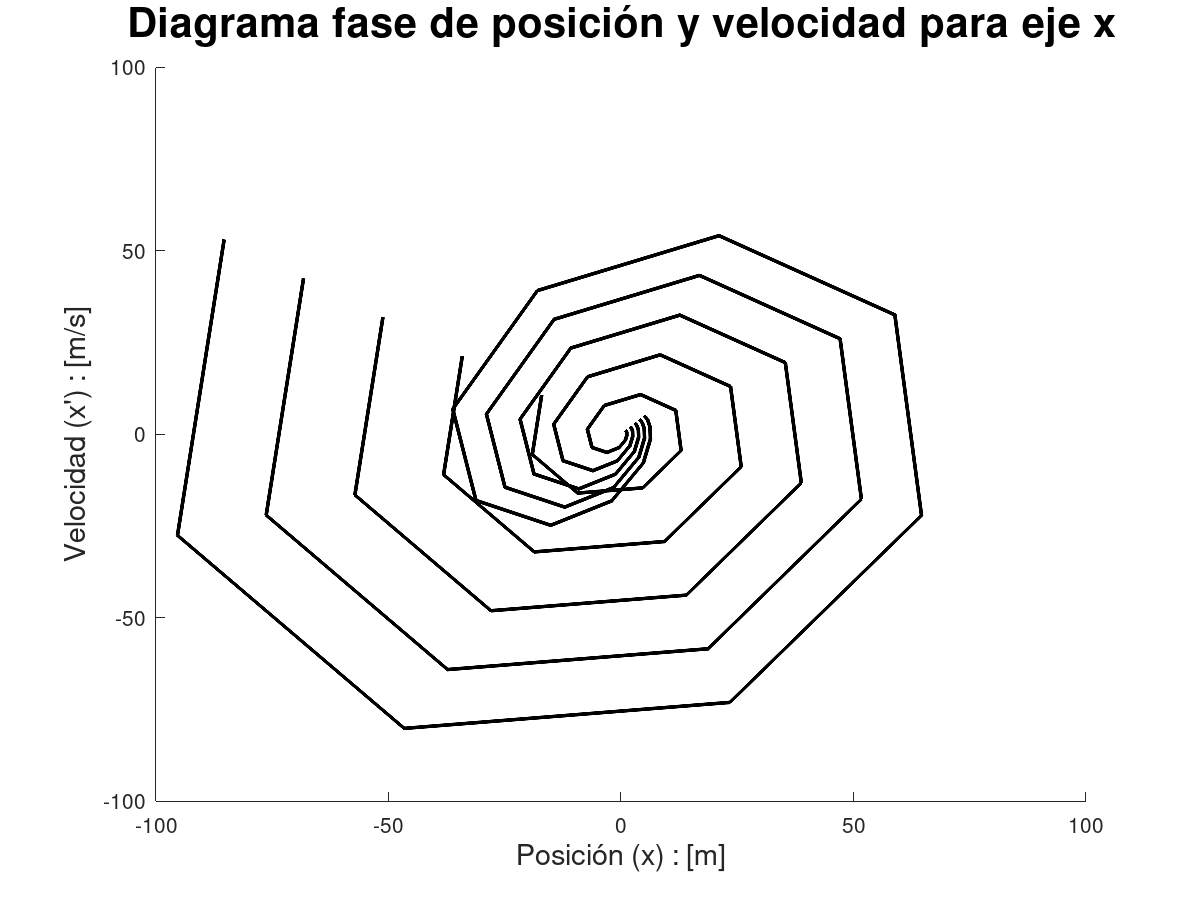
\includegraphics[scale=0.2]{img/fig10.png}
 % fig01.png: 1200x900 px, 72dpi, 42.33x31.75 cm, bb=0 0 1200 900
 \caption{Diagrama fase de $x(t)$ y $\dot{x}(t)$.}
\end{figure}

\begin{figure}
 \centering
 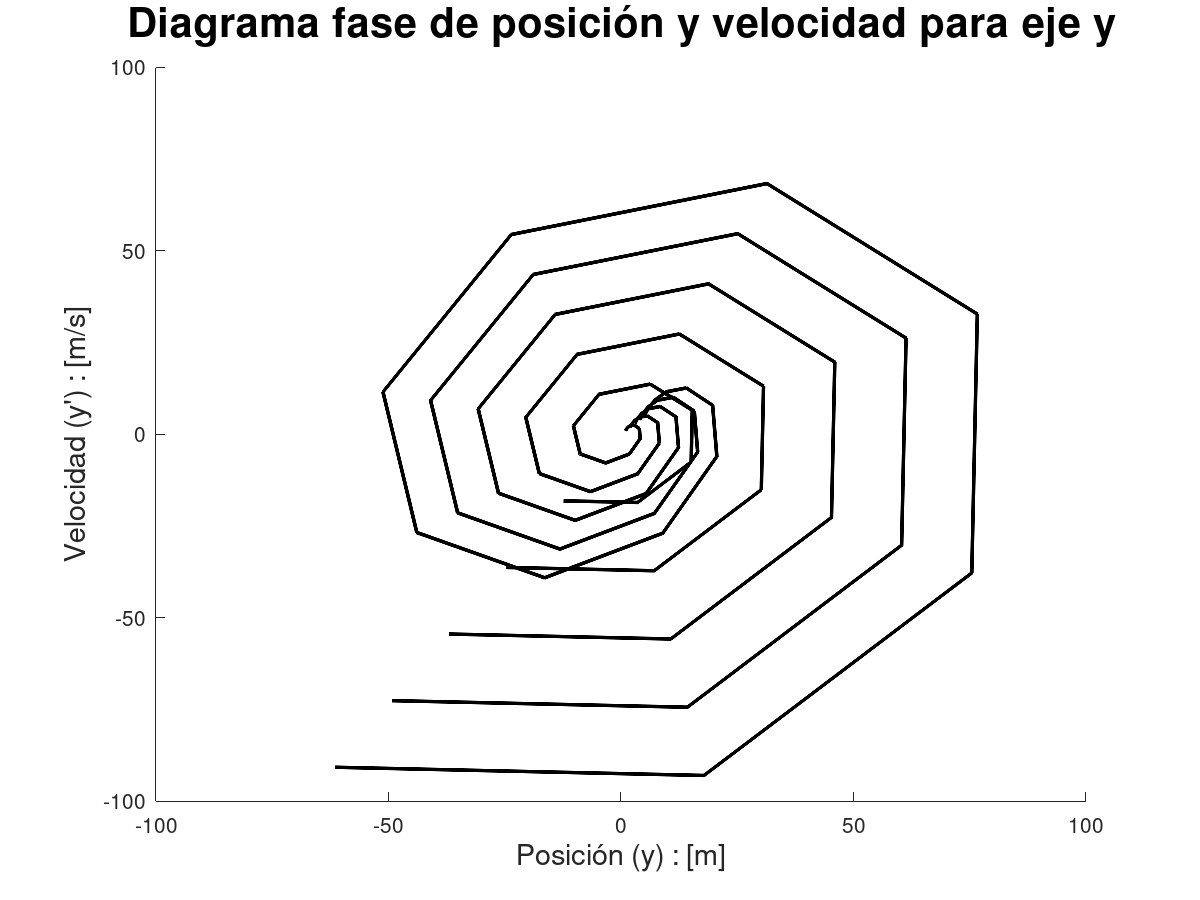
\includegraphics[scale=0.2]{img/fig11.png}
 % fig01.png: 1200x900 px, 72dpi, 42.33x31.75 cm, bb=0 0 1200 900
 \caption{Diagrama fase de $y(t)$ y $\dot{y}(t)$.}
\end{figure}

\begin{figure}
 \centering
 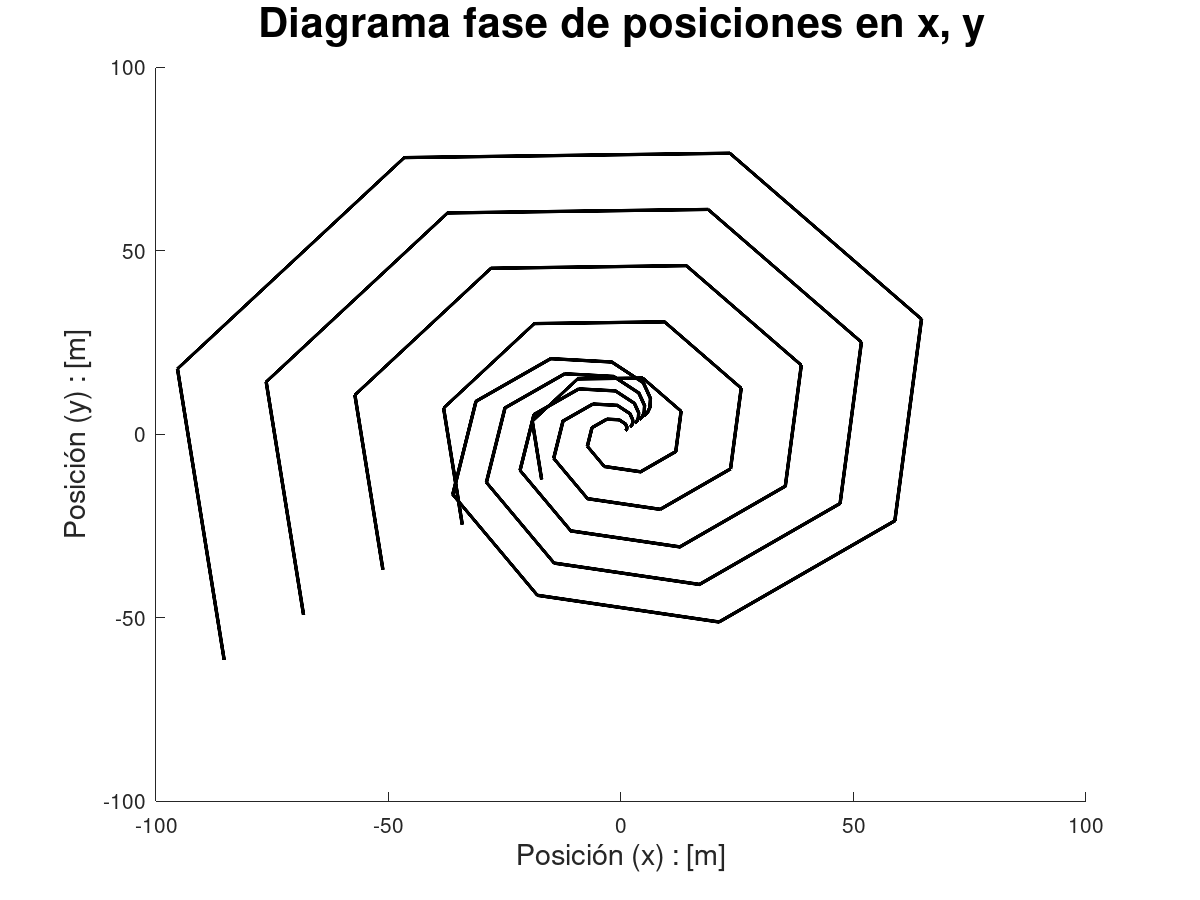
\includegraphics[scale=0.2]{img/fig12.png}
 % fig01.png: 1200x900 px, 72dpi, 42.33x31.75 cm, bb=0 0 1200 900
 \caption{Diagrama fase de $x(t)$ y $y(t)$.}
\end{figure}





\end{document}
